\section{OntoGEM} % Seções são adicionadas para organizar sua apresentação em blocos discretos, todas as seções e subseções são automaticamente exibidas no índice como uma visão geral da apresentação, mas NÃO são exibidas como slides separados.

%----------------------------------------------------------------------------------------
%----------------------------------------------------------------------------------------

\begin{frame}{OntoGEM}
	\begin{itemize}
		\item O processo de construção de um modelo computacional do metabolismo de um organismo é conhecido
		como \textbf{reconstrução}, enquanto o modelo resultante é frequentemente denominado \textbf{modelo metabólico em
			escala genômica (GEM)}.
		\item Durante o processo de reconstrução, especialistas do domínio precisam revisar diferentes banco de dados e a literatura respondendo perguntas como:
		\begin{itemize}
			\item \textit{Quais são os substratos da reação \textbf{R}}?
			\item \textit{Quais representações alternativas existem para a reação \textbf{R}?}
		\end{itemize}
		\item  Souza, N. A. de (2025) construiu a ontologia OntoGEM com o apoio de especialistas de domínio para facilitar o processo de reconstrução e de resolução das perguntas
	\end{itemize}     
\end{frame}

%----------------------------------------------------------------------------------------

\begin{frame}{OntoGEM}
	\begin{figure}[H]
		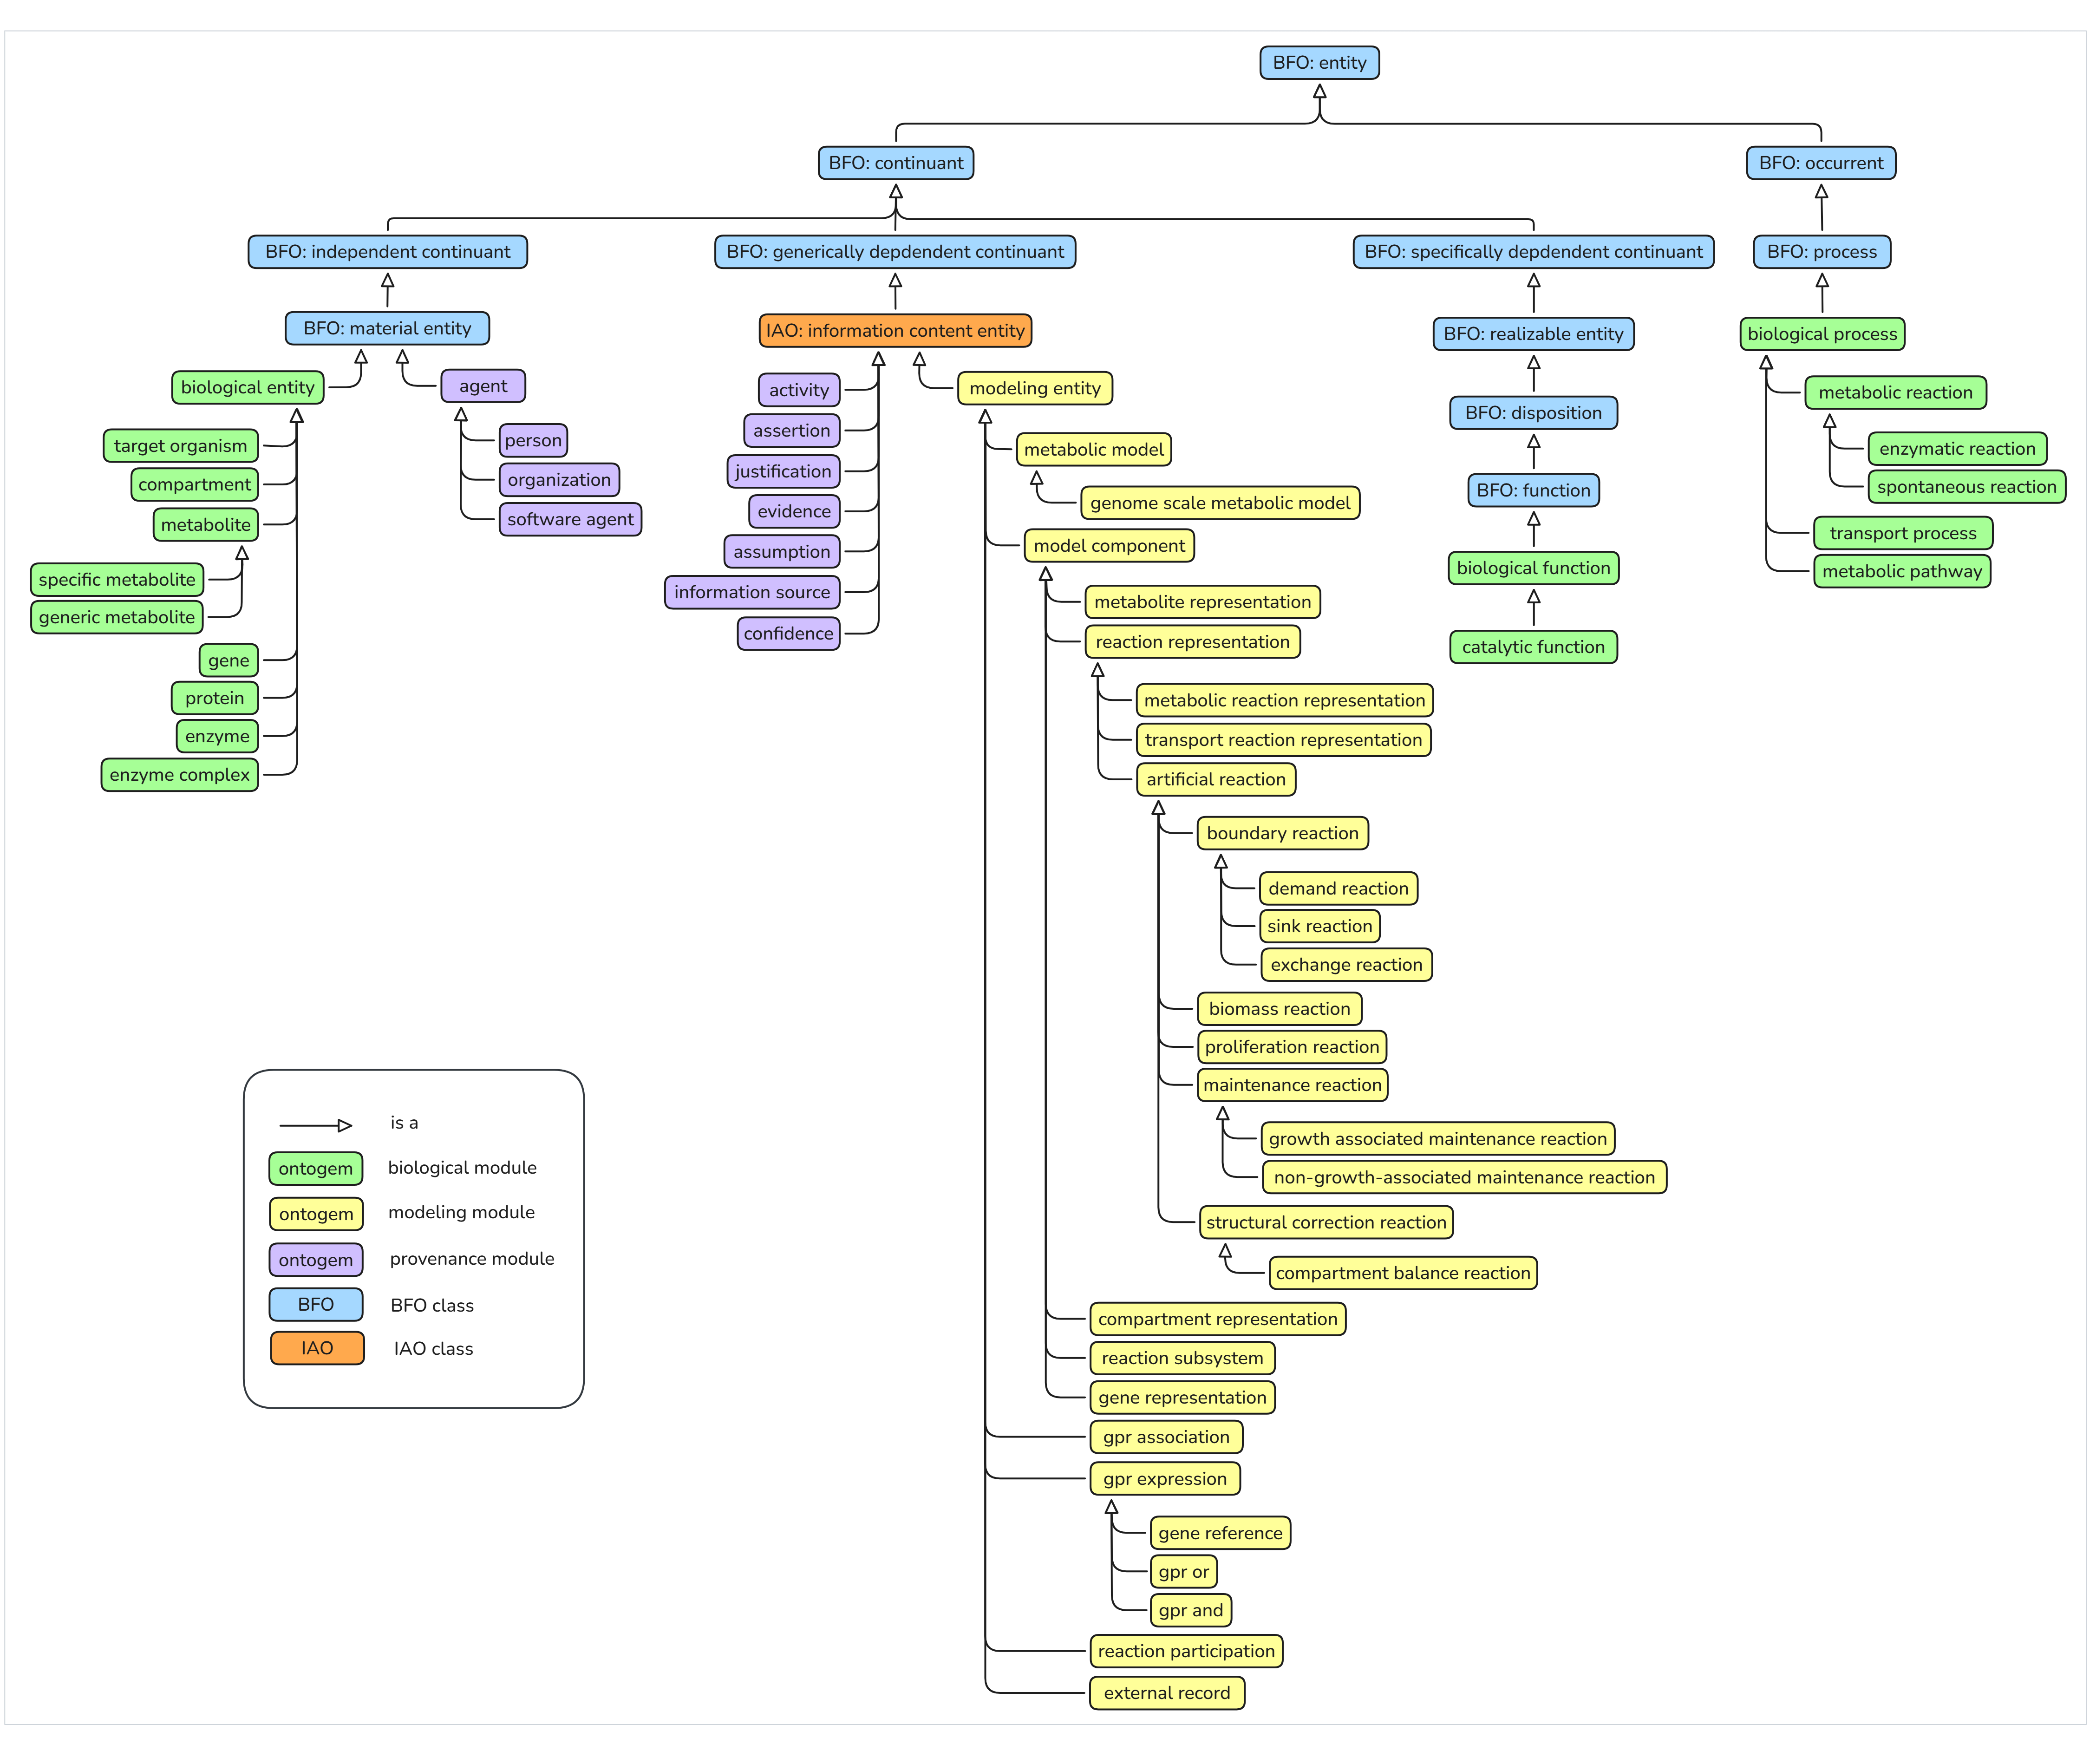
\includegraphics[width=0.70\linewidth]{img/new-relations-ontogem.png}
	\end{figure}
\end{frame}

